\section{Architectural design}

\subsection{Overview}

\begin{figure}[h!]
	\centering
	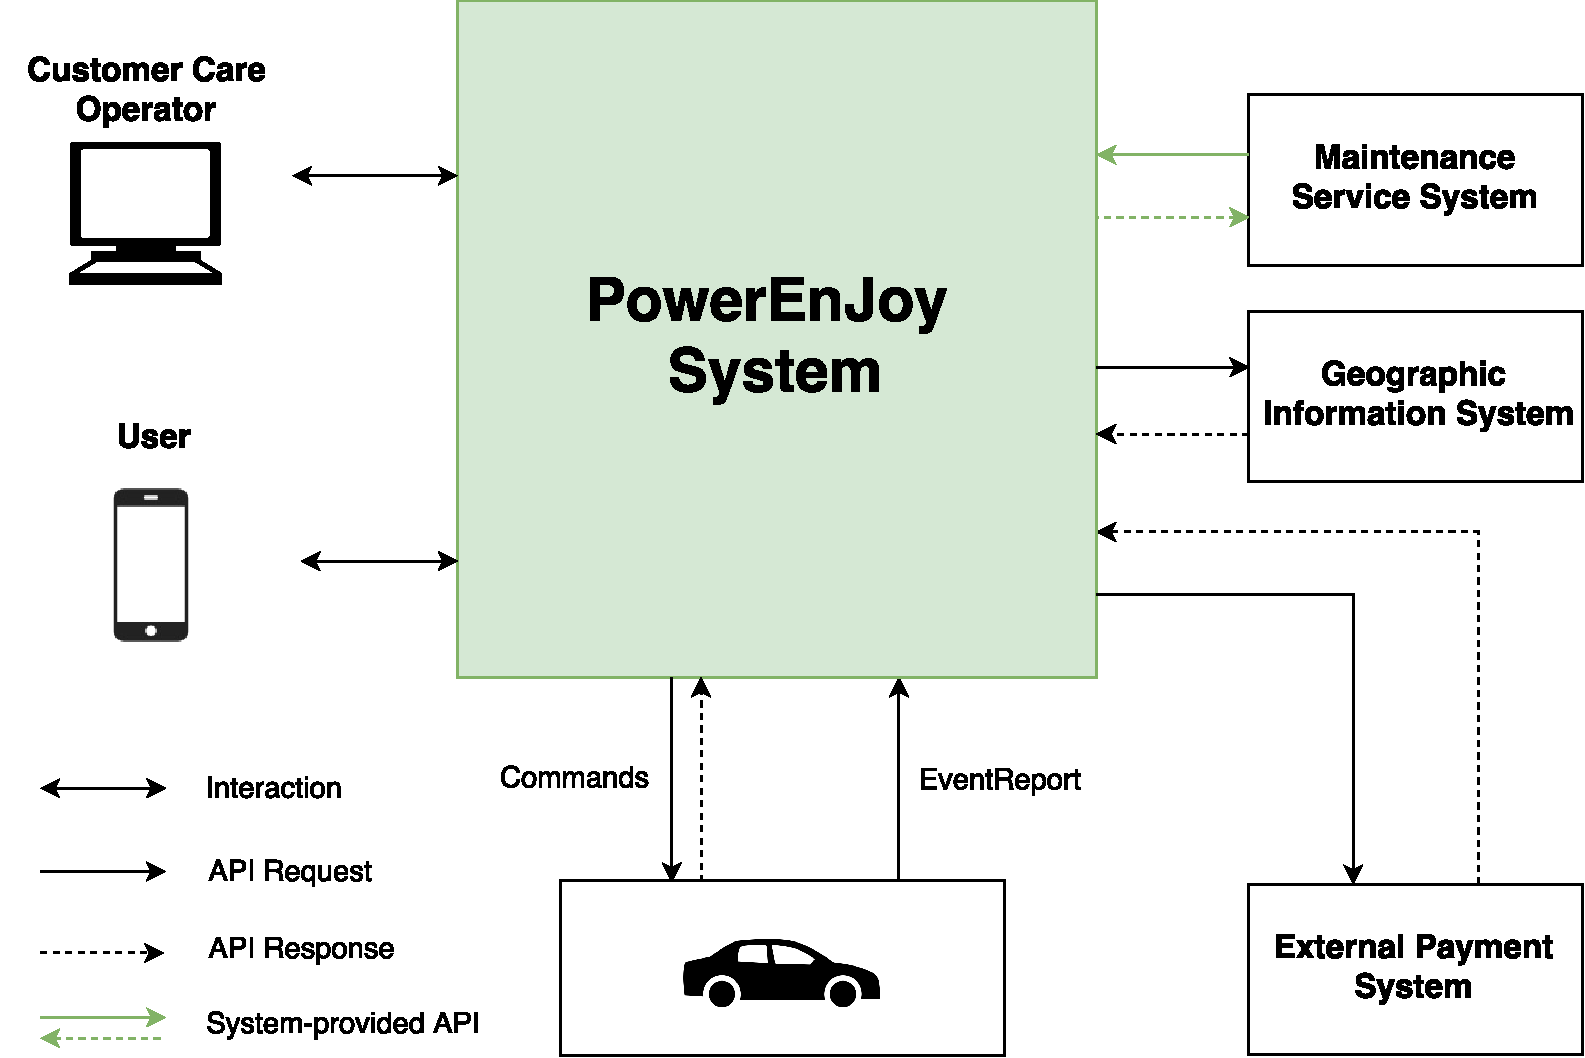
\includegraphics[width=\linewidth]{contextViewPoint}
	\caption{
		\label{fig:contextViewPoint} 
		Context viewpoint
	}
\end{figure}
\clearpage



We need to design a system which allows communications with many agents such as cars, users, external systems, etc.
Moreover we recognize that in most of the interactions the system is providing a service to agents so, after taking in consideration different alternatives, we decided to use a client-server architectural approach.

Cars offer to the system a set of primitives which allow it to interact with them: in this case it is clear that cars are providing the system services, so they can be identified as serves while the system acts as a client; on the other end the notification functionality offered by cars clearly yields to an event-based approach due to the asynchronous nature of such interactions, this lead us to use a publish-subscribe paradigm for these specific interactions.

\subsection{Component view}
\begin{figure}[h!]
	\centering
	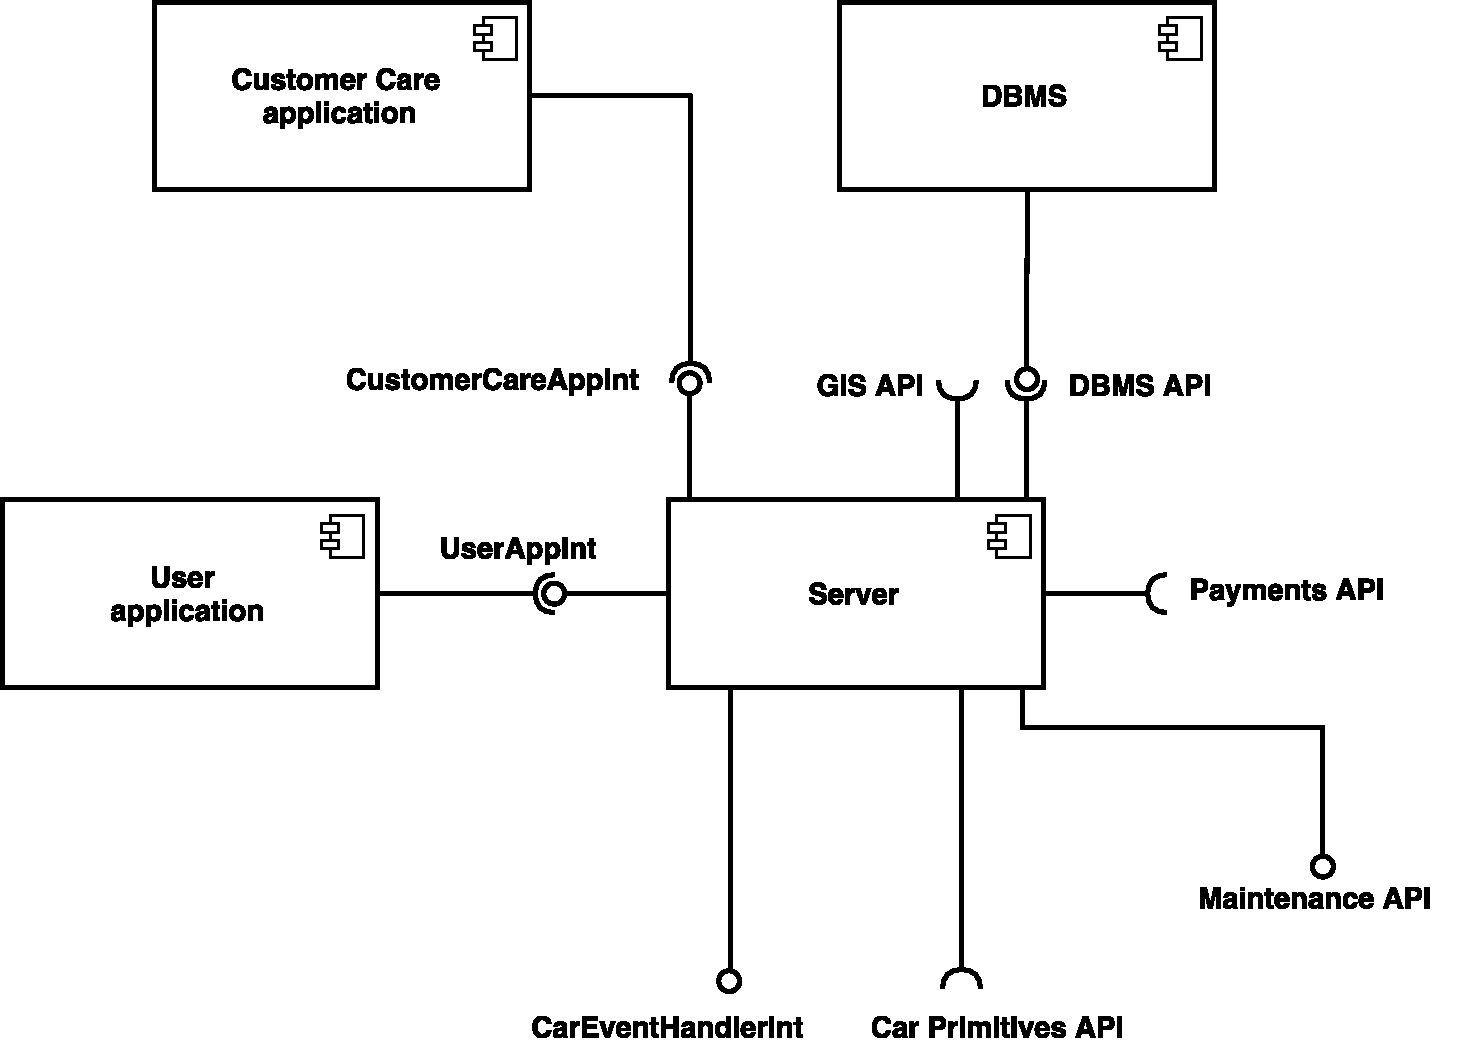
\includegraphics[width=\linewidth]{highLevelComponents}
	\caption{
		\label{fig:highLevelComponents} 
		High-level components
	}
\end{figure}
Considering all the previous graphs, we have identified in \autoref{fig:highLevelComponents} the following high level components, interfaces and mapping of the functionality defined in the RASD:
\begin{itemize}

	\item User application
	\begin{itemize}
		\item Register
		\item Login
		\item View the map with the position of
		\begin{itemize}
			\item himself
			\item safe areas
			\item available cars (with their battery level)
			\item charging stations
		\end{itemize}
		\item Reserve a car
		\item View customer care contacts
		\item Unlock the reserved car
		\item View and edit personal information
		\item View rents and payments history
	\end{itemize}
	
	\item Customer Care application
	\begin{itemize}
		\item View each user profile, including personal information, rent and payments history\todo{current rent?}
		\item Mark and unmark users as banned
		\item Mark cars as Not Available
	\end{itemize}
	
	\item DBMS
	\begin{itemize}
		\item Store and retrieve data
	\end{itemize}	
	
	\item GIS API
	\begin{itemize}
		\item Get a map which will be populated with markers
	\end{itemize}
	
	\item Payments API
	\begin{itemize}
		\item Execute payment transactions
	\end{itemize}
	
	\item Maintenance API
	\begin{itemize}
		\item Expose the list of the cars tagged as Not Available with their GPS position and a brief description of the problem
		\item Tag Not Available cars as Available
	\end{itemize}
	
	\item Car Primitives API
	\begin{itemize}
		\item Call car embedded system's primitives
	\end{itemize}
	
	\item Car Event Handler Interface \todo{name must be consistent with graph}
	\begin{itemize}
		\item Triggered by an event notification from cars
	\end{itemize}
\end{itemize}

\subsection{Deployment view}
\subsection{Runtime view}
\subsection{Component interfaces}
\subsection{Architectural style and patterns}
\subsection{Other design decision}